\chapter{Conception et architecture du système}
\label{chap:conception}

\section{Gestion du projet (Méthodologie Agile)}

Dans le cadre de ce projet, nous avons adopté une méthodologie Agile de type Scrum afin de permettre une évolution itérative et progressive du système.

\subsection{Product Backlog}

Le Product Backlog regroupe l’ensemble des fonctionnalités à développer, exprimées sous forme de User Stories.

\begin{table}[H]
\centering
\begin{tabular}{|c|p{10cm}|c|}
\hline
\textbf{ID} & \textbf{User Story} & \textbf{Priorité} \\
\hline
US1 & En tant qu'utilisateur, je peux uploader un fichier EDF afin d'analyser un enregistrement PSG & Haute \\
\hline
US2 & En tant que système, je peux segmenter le signal en époques de 30 secondes & Haute \\
\hline
US3 & En tant que système, je peux classifier les stades du sommeil (Wake, NREM, REM) & Haute \\
\hline
US4 & En tant qu'utilisateur, je peux visualiser l'hypnogramme généré & Haute \\
\hline
US5 & En tant qu'utilisateur, je peux comparer les prédictions avec un hypnogramme réel & Haute \\
\hline
US6 & En tant qu'utilisateur, je peux visualiser les signaux EEG, EOG et EMG & Moyenne \\
\hline
US7 & En tant que système, je peux générer des explications (SHAP, attention, saliency) & Haute \\
\hline
US8 & En tant qu'utilisateur, je peux exporter les résultats (PDF, CSV) & Moyenne \\
\hline
US9 & En tant que système, je peux stocker les résultats dans une base de données & Moyenne \\
\hline
US10 & En tant qu'utilisateur, je peux naviguer entre les époques et consulter les détails & Haute \\
\hline
\end{tabular}
\caption{Product Backlog du projet}
\end{table}

\subsection{Planification des Sprints}

Le projet a été divisé en plusieurs sprints de durée de deux semaines chacun, permettant une progression incrémentale.

\subsubsection{Sprint 1 : Préparation des données}

\begin{itemize}
    \item Chargement des fichiers EDF
    \item Prétraitement des signaux
    \item Segmentation en époques
\end{itemize}

\subsubsection{Sprint 2 : Modélisation}

\begin{itemize}
    \item Implémentation du modèle LSTM
    \item Entraînement sur les données SHHS
    \item Évaluation des performances
\end{itemize}

\subsubsection{Sprint 3 : Amélioration et Explicabilité}

\begin{itemize}
    \item Intégration des techniques SHAP
    \item Ajout du mécanisme d'attention
    \item Analyse des résultats
\end{itemize}

\subsubsection{Sprint 4 : Interface utilisateur}

\begin{itemize}
    \item Développement de l’interface web
    \item Visualisation des signaux
    \item Affichage de l’hypnogramme
\end{itemize}

\subsubsection{Sprint 5 : Intégration et Tests}

\begin{itemize}
    \item Intégration du backend et frontend
    \item Tests fonctionnels
    \item Validation globale du système
\end{itemize}

\subsection{Avantages de l'approche Agile}

L’adoption de la méthodologie Agile a permis :

\begin{itemize}
    \item Une meilleure gestion des priorités
    \item Une adaptation continue aux besoins
    \item Une livraison progressive des fonctionnalités
    \item Une amélioration continue du système
\end{itemize}

\section{Vue d’ensemble}

Le système XAI-Sleep suit une architecture client-serveur modulaire (Figure~\ref{fig:archi}).

\begin{figure}[H]
\centering
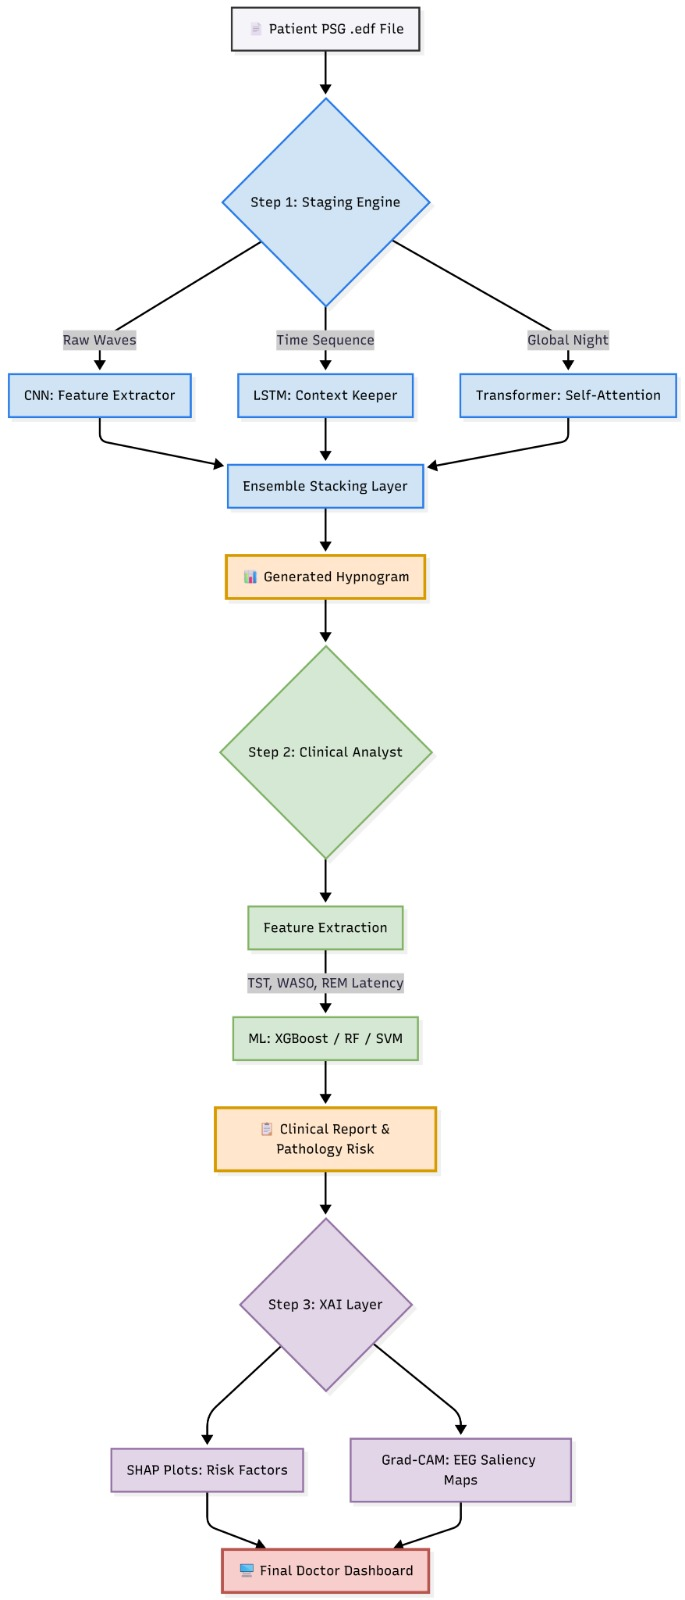
\includegraphics[width=0.7\textwidth]{images/architecture.jpeg}
\caption{Architecture globale du système}
\label{fig:archi}
\end{figure}

Les principaux composants sont :
\begin{itemize}
\item \textbf{Backend} : API FastAPI, modèle d’ensemble, moteur d’explications.
\item \textbf{Frontend} : application web React (ou Streamlit) pour l’interaction.
\item \textbf{Base de données} : PostgreSQL pour stocker les résultats.
\item \textbf{CI/CD} : GitHub Actions, Docker, Kubernetes.
\end{itemize}

\section{Modèle d’ensemble (stacking)}

\subsection{Modèles de base}
\begin{itemize}
\item \textbf{CNN} : 3 blocs convolutifs (filtres 32,64,128) suivis de global average pooling.
\item \textbf{LSTM} : 2 couches LSTM bidirectionnelles de 128 unités chacune.
\item \textbf{Transformer} : encodeur avec 4 têtes d’attention et dimension 128.
\end{itemize}
Chaque modèle prend en entrée des épisodes de 30 secondes (3000 échantillons) des deux canaux EEG (Fpz-Cz, Pz-Oz) ou 5 EEG (Fpz-Cz, Pz-Oz ou sec), EOG (R,L) et EMG canaux  . Les sorties (logits ou probabilités) sont concaténées.

\subsection{Méta-apprenant avec LCS}
Le méta-apprenant est un réseau de neurones à 2 couches cachées. Un \textbf{lissage contextuel localisé} (LCS) est appliqué après la prédiction : il utilise une fenêtre glissante (taille 5) pour lisser les transitions aberrantes (par ex. W→REM→W), en s’appuyant sur les probabilités et les règles cliniques (interdiction des transitions impossibles).

\section{Moteur d’explicabilité}

Pour chaque modèle de base et pour l’ensemble, plusieurs méthodes sont disponibles :

\begin{itemize}
\item \textbf{SHAP} : calcul des valeurs SHAP sur l’ensemble des caractéristiques (moyenne par canal).
\item \textbf{Attention} : extraction des poids d’attention du LSTM et du Transformer.
\item \textbf{Saliency} : gradient de la sortie par rapport à l’entrée pour le CNN.
\end{itemize}

Ces explications sont fusionnées dans un tableau de bord interactif.

\section{Interface utilisateur}

L’interface web (Figure~\ref{fig:interface}) permet :
\begin{itemize}
\item Téléchargement d’un fichier EDF.
\item Visualisation des signaux bruts.
\item Affichage de l’hypnogramme prédit.
\item Navigation épisode par épisode avec explications (SHAP, attention).
\item Export PDF/JSON.
\end{itemize}

\begin{figure}[H]
\centering
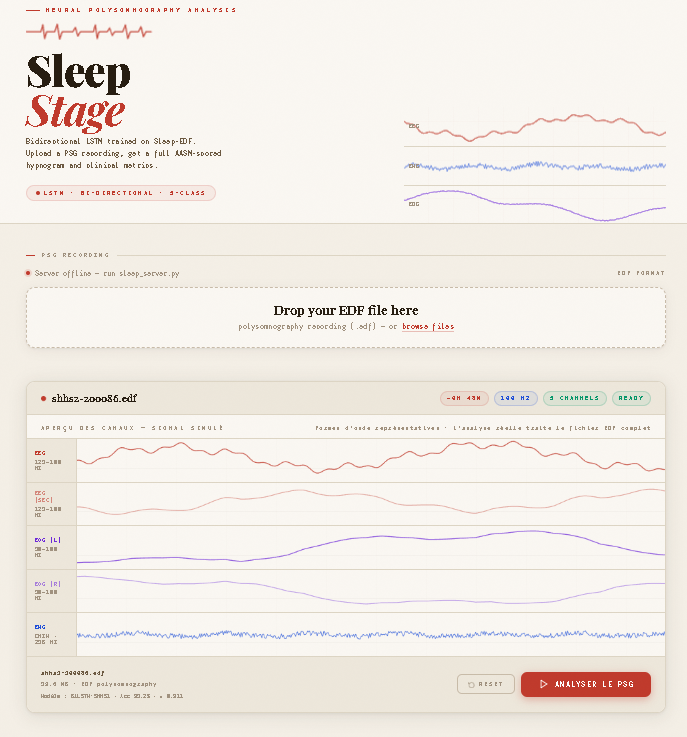
\includegraphics[width=0.7\textwidth]{images/interfaceWeb.png}
\caption{Maquette de l’interface utilisateur}
\label{fig:interface}
\end{figure}

\section{Automatisation du déploiement}

Une pipeline CI/CD avec GitHub Actions construit une image Docker de l’application, l’exécute sur un cluster Kubernetes (minikube en développement, cloud en production). Les tests unitaires et d’intégration sont automatisés.